\subsection{Historia de la luz y sus teorías}

Antes de comenzar con el tema, veamos un breve resumen de la historia de la luz y sus teorías. Esto nos va a servir para saber qué entendemos por luz y por qué no vamos a usar las ecuaciones de onda del capitulo pasado.

\subsubsection{La teoría corpuscular de Newton}

A finales del siglo XVII, Isaac Newton propuso que la luz estaba compuesta por pequeños corpúsculos (partículas). Esta teoría corpuscular explicaba bien la reflexión y la refracción: al considerar que las partículas de luz eran atraídas por los medios más densos, se podía justificar el cambio de dirección (ley de Snell). Newton también contaba con gran autoridad científica, por lo que su modelo prevaleció durante mucho tiempo.

\subsubsection{La teoría ondulatoria de Huygens}

\begin{wrapfigure}{r}{0.25\textwidth}
  \centering
  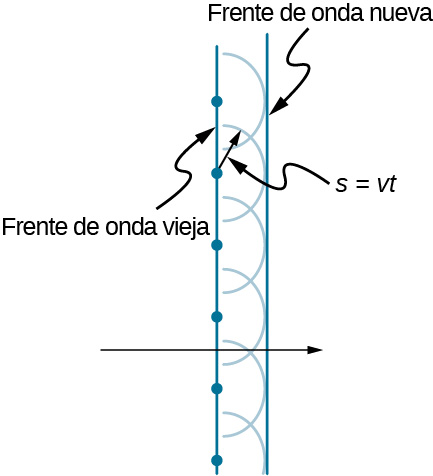
\includegraphics[width=\linewidth]{huygens_principle.jpg}
  \caption{Principio de Huygens}
  \label{fig:huygens_principle}
\end{wrapfigure}
Casi en paralelo, Christiaan Huygens (1678) propuso una teoría alternativa: la teoría ondulatoria de la luz. En lugar de partículas, la luz sería una perturbación en un medio elástico invisible ``el éter'' propagándose como ondas. Huygens explicó la refracción como resultado de velocidades distintas de propagación en diferentes medios y formuló el principio de Huygens, según el cual cada punto de un frente de onda es fuente de nuevas ondas secundarias.

Ambas teorías tenían fortalezas: Newton explicaba bien la geometría de los rayos y el fenómeno de la reflexión, mientras que Huygens ofrecía una mejor descripción de la difracción y la interferencia, fenómenos que aún no se habían explorado completamente.

Puedes leer más sobre este principio en OpenStax (\cite{openstax}: \href{https://openstax.org/books/f%C3%ADsica-universitaria-volumen-3/pages/1-6-principio-de-huygens}{Volumen 3, Principio de Huygens}).

\subsubsection{El renacimiento de la teoría ondulatoria}

A inicios del siglo XIX, los experimentos de Thomas Young (interferencia de doble rendija, 1801) y Augustin-Jean Fresnel (difracción) ofrecieron evidencia concluyente a favor de la teoría ondulatoria. Estos fenómenos no podían explicarse con partículas individuales, ya que mostraban patrones de superposición característicos de ondas. La luz se empezó a entender como una onda transversal, propagándose en el éter.

\subsubsection{Maxwell y el electromagnetismo}
\label{sec:maxwell_electromagnetismo}

Entre 1861 y 1865, James Clerk Maxwell formuló un sistema de ecuaciones que unificaba los fenómenos eléctricos y magnéticos: las ecuaciones de Maxwell. Al analizarlas, dedujo que las ondas electromagnéticas se propagaban en el vacío a una velocidad determinada por las constantes eléctricas y magnéticas del medio:

\[
v = \frac{1}{\sqrt{\mu_0 \varepsilon_0}} = \lambda f \approx 3 \times 10^8 \ \text{m/s}
\]

Esta velocidad coincidía exactamente con la de la luz. De este modo, la luz fue identificada como una onda electromagnética. Esto fue un triunfo de la teoría ondulatoria y de la física clásica. Sin embargo, las ecuaciones de Maxwell predecían \textbf{energía propagada} de forma continua, sin cuantización.

La figura \ref{fig:ond_electromagnetica} muestra una onda electromagnética. Vea que es una perturbación del campo eléctrico \(\vec{E}\) y del campo magnético \(\vec{B}\). Ambos son perpendiculares entre sí y también perpendiculares a la dirección de propagación de la onda.

\begin{figure}[ht]
  \centering
  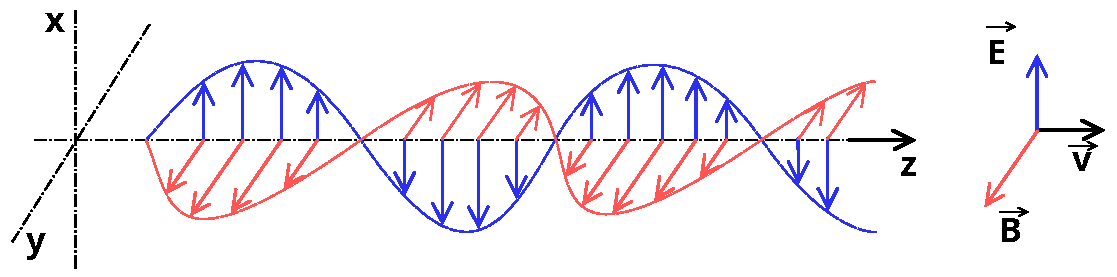
\includegraphics[width=0.8\textwidth]{electromagnetic_wave.pdf}
  \caption{Representación de una onda electromagnética.}
  \label{fig:ond_electromagnetica}
\end{figure}

El hecho de que las perturbaciones del campo eléctrico \(\vec{E}\) y del campo magnético \(\vec{B}\) en una onda electromagnética sean ortogonales (perpendiculares entre sí y a la dirección de propagación) no es un axioma ni una suposición: es una consecuencia directa de las ecuaciones de Maxwell en el vacío.

\paragraph{Demostración}

Consideremos una onda electromagnética plana que se propaga en el vacío en la dirección \(x\). Entonces buscamos soluciones de las ecuaciones de Maxwell donde los campos \(\vec{E}\) y \(\vec{B}\) dependen solo de \(x\) y del tiempo \(t\).

Queremos demostrar que:
\begin{itemize}
  \item \(\vec{E} \perp \vec{B}\)
  \item \(\vec{E} \perp \vec{k}\), donde \(\vec{k}\) es el vector de propagación (por ejemplo, en la dirección \(x\)).
\end{itemize}

Recordemos las ecuaciones de Maxwell en ausencia de cargas y corrientes (\(\rho = 0\), \(\vec{J} = 0\)):
\begin{align*}
  \nabla \cdot \vec{E} &= 0 \\
  \nabla \cdot \vec{B} &= 0 \\
  \nabla \times \vec{E} &= -\frac{\partial \vec{B}}{\partial t} \\
  \nabla \times \vec{B} &= \mu_0 \varepsilon_0 \frac{\partial \vec{E}}{\partial t}
\end{align*}

Vamos a usar estas ecuaciones para deducir la orientación relativa entre \(\vec{E}\), \(\vec{B}\), y la dirección de propagación.

Buscamos soluciones del tipo:

\[
\vec{E}(x,t), \quad \vec{B}(x,t)
\]

Asumamos que \(\vec{E}\) apunta en la dirección \(y\), y \(\vec{B}\) en la dirección \(z\):

\[
\vec{E} = E_y(x,t)\, \hat{y}, \quad \vec{B} = B_z(x,t)\, \hat{z}
\]

Dirección de propagación: \(\vec{k} = k\, \hat{x}\)

La tercera ecuación de Maxwell (ecuación de Faraday) nos dice que una variación en el campo magnético genera un campo eléctrico:
\[
\nabla \times \vec{E} = -\frac{\partial \vec{B}}{\partial t}
\]
El rotacional de \(\vec{E} = E_y(x,t)\, \hat{y}\) tiene solo una componente en \(z\):
\[
\nabla \times \vec{E} = \left( \frac{\partial E_y}{\partial x} \right) \hat{z}
\]
Entonces:
\[
\left( \nabla \times \vec{E} \right)_z = \frac{\partial E_y}{\partial x} = -\frac{\partial B_z}{\partial t}
\]

Este resultado indica que una variación del campo eléctrico \(E_y\) en la dirección de propagación \(x\) genera una variación temporal del campo magnético \(B_z\). Además, como las componentes están en direcciones ortogonales, se confirma que \(\vec{E} \perp \vec{B}\).

Análogamente, aplicamos la cuarta ecuación de Maxwell (ecuación de Maxwell-Ampère):
\[
\nabla \times \vec{B} = \mu_0 \varepsilon_0 \frac{\partial \vec{E}}{\partial t}
\]
Esta ecuación nos dice que una variación temporal del campo eléctrico genera un campo magnético.

El rotacional de \(\vec{B} = B_z(x,t)\, \hat{z}\) tiene componente en \(y\):
\[
\nabla \times \vec{B} = -\left( \frac{\partial B_z}{\partial x} \right) \hat{y}
\]
Entonces:
\[
\left( \nabla \times \vec{B} \right)_y = -\frac{\partial B_z}{\partial x} = \mu_0 \varepsilon_0 \frac{\partial E_y}{\partial t}
\]
Lo cual también es coherente con lo anterior.

\paragraph{Conclusión geométrica}

Los campos cumplen las siguientes condiciones:
\begin{itemize}
  \item \(\vec{E} \perp \vec{B}\), porque sus componentes son ortogonales \(y\) y \(z\),
  \item \(\vec{E} \perp \vec{k}\) y \(\vec{B} \perp \vec{k}\), porque ninguno depende de la componente \(x\) directamente.
\end{itemize}
Además, por el producto vectorial:
\[
\vec{E} \times \vec{B} \propto \vec{k}
\]
Es decir, la dirección de propagación es perpendicular a ambos campos, y se define por el producto vectorial de los campos.

Si la onda se propaga hacia la dirección \(x\):
\begin{itemize}
  \item \(\vec{E}\) oscila sobre el eje \(y\),
  \item \(\vec{B}\) oscila sobre el eje \(z\),
  \item La energía fluye en la dirección de \(\vec{E} \times \vec{B} = \hat{x}\).
\end{itemize}

\subsubsection{Crisis en la física clásica: la radiación del cuerpo negro}

A fines del siglo XIX, al estudiar la radiación del cuerpo negro, los físicos encontraron que la ley de Rayleigh-Jeans (derivada desde los supuestos clásicos) predecía una divergencia ultravioleta: una cantidad infinita de \textbf{energía}\footnote{Es importante que vea que el problema fue la \textbf{energía} que se emitía de forma continua, no el modelo ondulatorio. Ver la radiación electromagnética como onda es correcto, pero la energía que se emite de forma continua no lo es.} en las frecuencias altas, lo que claramente no ocurría en la realidad.

Para resolver esta contradicción, en 1900, Max Planck introdujo una hipótesis revolucionaria: la energía de la radiación electromagnética no se emite ni se absorbe de manera continua, sino en cuantos discretos, proporcionales a la frecuencia:

\begin{equation}
  E = h f
  \label{eq:planck}
\end{equation}
donde \(h=6.626 \times 10^{-34} \ \text{[Js]}\) es la constante de Planck. Este ajuste fue inicialmente visto como una herramienta matemática, no como una descripción física profunda.

\subsubsection{Einstein y el efecto fotoeléctrico: nacimiento del fotón}

En 1905, Albert Einstein retomó y radicalizó la idea de Planck para explicar el efecto fotoeléctrico que es el fenómeno por el cual un material emite electrones cuando es iluminado por luz. Este efecto fue observado experimentalmente desde finales del siglo XIX, pero no podía ser explicado mediante la teoría electromagnética clásica.

\begin{wrapfigure}{r}{0.3\textwidth}
  \centering
  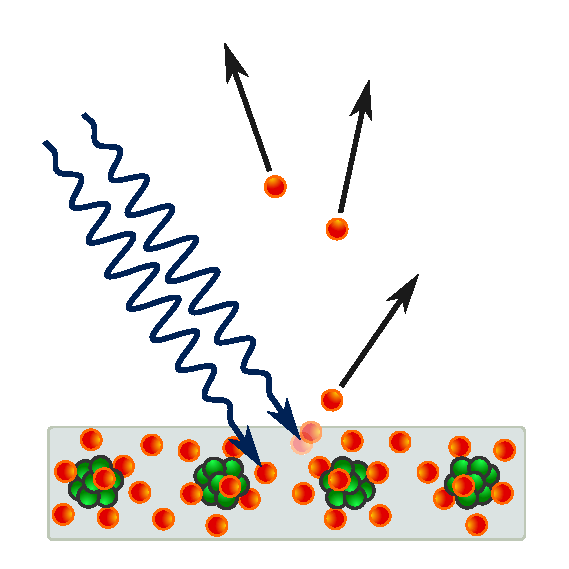
\includegraphics[width=\linewidth]{photoelectric_effect.pdf}
  \caption{Experimento típico: Se ilumina la superficie de un metal con luz de frecuencia conocida.}
  \label{fig:photoelectric_effect}
\end{wrapfigure}
Como se ve en la figura \ref{fig:photoelectric_effect} un experimento típico del efecto fotoeléctrico consiste en iluminar una placa metálica cargada eléctricamente con luz de una frecuencia conocida. Cuando se hace esto se observa que:
\begin{itemize}
  \item A frecuencias bajas, no se emiten electrones, sin importar cuán intensa sea la luz.
  \item A frecuencias suficientemente altas, sí se emiten electrones, incluso si la intensidad de la luz es débil.
  \item Si se aumenta la frecuencia de la luz por encima de cierto umbral, los electrones emitidos tienen mayor energía cinética.
\end{itemize}

Según la teoría clásica de ondas electromagnéticas, la energía asociada a las ondas como vimos en la sección \ref{sec:wave_energy} depende de la intensidad (\(I=P/S\)), entonces, la energía de la luz debería depender de la intensidad, no de la frecuencia. Es decir, una luz intensa debería poder arrancar electrones sin importar su frecuencia, dado suficiente tiempo.

Sin embargo, los experimentos mostraban lo contrario: una luz de baja frecuencia nunca arrancaba electrones, por más intensa que fuera. Esto no tenía explicación dentro del marco clásico.

Einstein propuso que la luz estaba compuesta de cuantos de energía localizados: fotones. Cada fotón tiene energía \(E = h f\), y al aplicar esta idea al efecto fotoeléctrico concluyó que un electrón dentro del metal solo puede absorber un fotón a la vez, y si ese fotón tiene suficiente energía, el electrón puede escapar del metal.

Para mayor elegancia formal se suele escribir usando la constante reducida \(\hbar = \frac{h}{2\pi}\), entonces:

\begin{equation*}
  E = \hbar \omega
\end{equation*}
donde \(\omega = 2\pi f\) es la frecuencia angular. Esta expresión es equivalente a la anterior.

\paragraph{La función de trabajo \(\phi\)}

Cada metal tiene una energía mínima necesaria para liberar un electrón de su superficie. Esta energía se llama función de trabajo y se denota con la letra griega \(\phi\):
\begin{equation*}
  \boxed{
    \phi = \text{energía mínima para extraer un electrón del metal}
  }
\end{equation*}

Entonces, si un fotón de energía \(E = h f\) incide sobre el metal:

\begin{itemize}
  \item Si \(h f < \phi\): no se emite ningún electrón (no importa la intensidad).
  \item Si \(h f \geq \phi\): el electrón es emitido y su energía cinética máxima es:
\end{itemize}

\begin{equation*}
  K_{\text{máx}} = \frac{1}{2} m_{e} v^2 = h f - \phi
\end{equation*}
donde \(m_e\) es la masa del electrón\footnote{Es muy importante que entienda que este efecto se cumple para los \textbf{electrones} (\(m_e = 9.11 \times 10^{-31} \ \text{kg}\)), no para protones, ya que se requiere muchisima más energía para arrancar un protón (\(m_p = 1.67 \times 10^{-27} \ \text{kg}\)).}. 

Este resultado coincide exactamente con los datos experimentales y contradice completamente las predicciones de la teoría clásica. Las implicaciones de esto son:

\begin{itemize}
  \item La energía de la luz está cuantizada.
  \item La intensidad de la luz afecta la cantidad de electrones emitidos, pero no su energía.
  \item Existe una frecuencia umbral \(f_0\) para cada metal, tal que si \(f < f_0\), no hay emisión fotoeléctrica.
\end{itemize}

Esta fue la primera evidencia directa de que la radiación electromagnética no solo tiene propiedades ondulatorias, sino también corpusculares.

Si quieres ver una prueba experimental del efecto fotoeléctrico, puedes ver el siguiente video: \href{https://youtu.be/oYnp0WZDhYQ?si=kIBH75DIIDv5hg_4}{YouTube: The Action Lab - The Photoelectric Effect}

\begin{tcolorbox}[myconclusion]
  En muchas ocaciones la energía se mide en electronvolti
\end{tcolorbox}

\subsubsection{Conclusión: dualidad onda-partícula}

El desarrollo culminó en la aceptación de que la luz posee una naturaleza dual: se comporta como onda en fenómenos de interferencia y difracción, y como partícula en fenómenos como el efecto fotoeléctrico y el efecto Compton. Esta dualidad se extiende a la materia misma, como demostraría De Broglie en 1924, sentando las bases para la mecánica cuántica. Para la materia Física II solo usaremos la deducción final del efecto fotoeléctrico y la ecuación de energía de Planck.